\subsection{Release}
  The release stage is the final stage in our workflow. This is when software gets released to the live environment and becomes available to partners. 
  \begin{figure}[H]
    \centering
    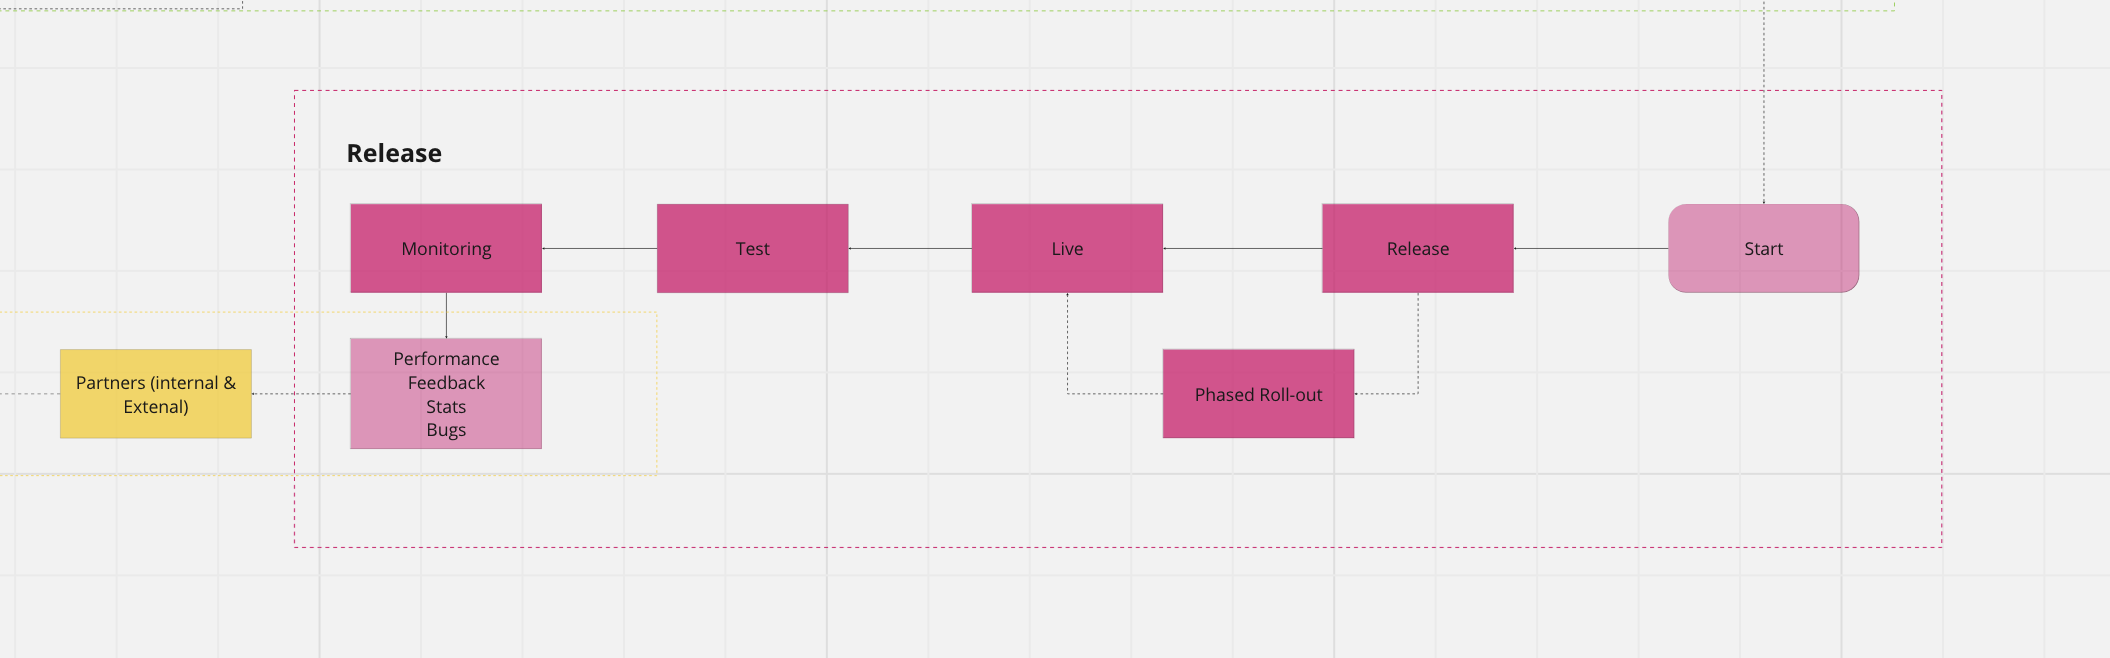
\includegraphics[width=8cm]{assets/workflow/release.png}
    \caption{Release stage of our ways of working.}
    \label{fig:workflowRelease}
  \end{figure}

  However in this case it doesn't become available to partners until we have confidence in the new system. We have config for each partner that 
  specifies what data they have access to. In the case of schedules, this includes keyspace information on where the data is retrieved from. As 
  previously discussed in the \hyperref[sec:cicd]{\textbf{Research}} section, the new and old system will run in parallel until our comparison tests 
  convince us that the new system outputs the same as the old.

  \begin{figure}[H]
    \centering
    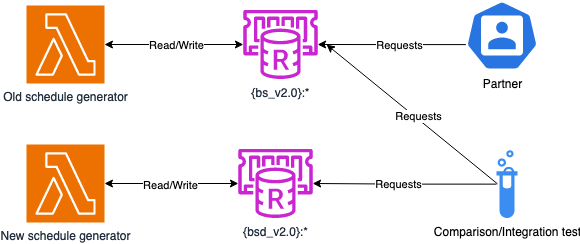
\includegraphics[width=8cm]{assets/keyspaceAccess.drawio.png}
    \caption{Diagram showing access to keyspaces.}
    \label{fig:keySpaceAccess}
  \end{figure}

  Until then partners will still access data from the old system, with a simple config change being the rollover/rollback mechanism. If we wanted we 
  could setup an automatic rollback and huddle system (Sathre, Zambreno, 2008), with the huddle portion consisting of developers being called out if 
  outside of working hours to monitor and remedy the situation. This can be done in many ways but one way would be through AWS alarm 
  actions (Amazon Web Services, 2024k). An alarm going into error would  triggers a rollback of the configs version in S3 (Amazon Web Services, 2024d).

  \begin{figure}[H]
    \centering
    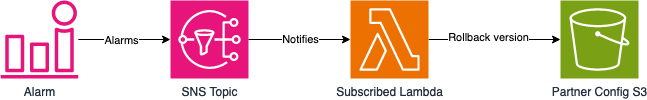
\includegraphics[width=8cm]{assets/rollback.drawio.png}
    \caption{Automatic rollback architecture on alarm error.}
    \label{fig:rollback}
  \end{figure}

  For our case this is most likely over-engineering and unnecessary. A config change only takes a minute to do and if there ever was an error we 
  would be notified and called out to fix the problem when necessary. 

  Once the switchover happens we wait for partner feedback and use created dashboards, these will be shown in the next section, to monitor 
  the new software. Alongside this, our comparison test and side-by-side running of new and old systems will continue for a short while after release, 
  allowing an easy rollback to the old system. Next this old lambdas scheduler will be disabled, but the lambda itself kept in case of an emergency. 
  Finally, after sufficient time has passed the old system can be deconstructed and removed completely.

\newpage
